\documentclass[12pt]{article}
\usepackage[margin=1in]{geometry}
\usepackage{times}
\usepackage{multicol}
\usepackage{setspace}
\usepackage{titlesec}
\usepackage{tikz}
\usepackage{hyperref}
\usetikzlibrary{calc,decorations.markings}

\titleformat{\section}{\normalfont\Large\bfseries}{\thesection}{1em}{}
\titleformat{\subsection}{\normalfont\large\bfseries}{\thesubsection}{1em}{}

\title{\textbf{Maxima–Minima Dialectics}\\\large Parliament Hill, Ottawa}
\author{}
\date{}

\begin{document}

% ---------- Cover Page ----------
\begin{titlepage}
\centering
\vspace*{2cm}

{\Huge \textbf{Maxima–Minima Dialectics}\par}
\vspace{0.5cm}
{\Large \textit{Parliament Hill, Ottawa}\par}

\vspace{2cm}

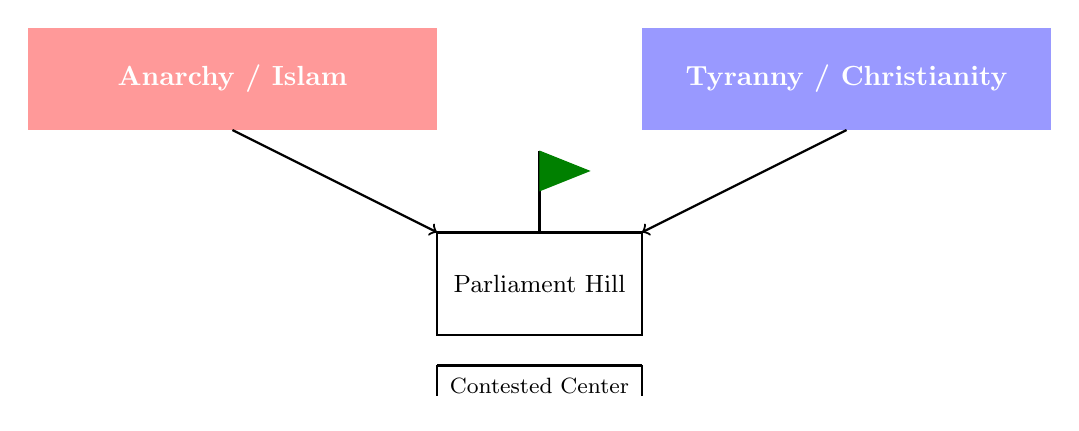
\begin{tikzpicture}[scale=1.3]
% Left banner - Minima
\fill[red!40] (-5,3) rectangle (-1,2);
\node[white, font=\bfseries] at (-3,2.5) {Anarchy / Islam};

% Right banner - Maxima
\fill[blue!40] (1,3) rectangle (5,2);
\node[white, font=\bfseries] at (3,2.5) {Tyranny / Christianity};

% Parliament Hill center
\draw[thick] (-1,0) rectangle (1,1);
\node at (0,0.5) {\small Parliament Hill};

% Flag pole
\draw[thick] (0,1) -- (0,1.8);
\fill[green!50!black] (0,1.8) -- (0.5,1.6) -- (0,1.4) -- cycle;

% Connecting lines
\draw[thick,->] (-3,2) -- (-1,1);
\draw[thick,->] (3,2) -- (1,1);

% Decorative base
\draw[thick] (-1,-0.3) -- (1,-0.3);
\draw[thick] (-1,-0.3) -- (-1,-0.6);
\draw[thick] (1,-0.3) -- (1,-0.6);
\node at (0,-0.5) {\footnotesize Contested Center};
\end{tikzpicture}

\vfill
{\small This document presents a mirrored pair — a \textit{Minima} (``Anarchy, Islam, and Canada'') and a \textit{Maxima Opposal} (``Tyranny, Christianity, and Canada'') — followed by a Hindu observer's bridge, a central axis meditation on Europe, and a final synthesis on infiltration and truth.}
\vspace*{2cm}
\end{titlepage}

% ---------- Page 1: Two-Column Dialectic ----------
\onehalfspacing
\begin{multicols}{2}

\section*{Anarchy, Islam, and Canada}
\noindent\textit{Revolving around Parliament Hill, Ottawa}

In the heart of Canada’s capital, Parliament Hill has become more than a symbolic seat of governance—it has become a theater where disparate ideologies, identities, and impulses converge. Anarchy, Islam, and Canada are not mere categories, but fluid forces that pulse through Ottawa’s streets, often in tension, sometimes in silence, and occasionally in eruption. The interplay between them—particularly as witnessed over the last few years—has recast Parliament Hill as both a sacred center and a contested frontier.

The era of \textit{Anarchy} surrounding the Freedom Convoy marked a rupture in the Canadian psyche. Before the Convoy, the idea of anarchy was theoretical, dormant, largely academic. Ottawa was a place of quiet routines and ceremonial politics. But when the trucks rolled in during the Freedom Convoy of 2022, anarchy stepped into the snow and parked itself in defiance of state order. The movement, catalyzed by vaccine mandates, spiraled into a deeper national catharsis about control, legitimacy, and belonging. Post-convoy, the embers of anarchy didn’t extinguish—they mutated. What remained was a shaken public consciousness, one that views Parliament Hill not as untouchable, but as penetrable, contestable.

\textit{Islam}’s visible arc in Ottawa intensified around \textit{The Palestinian Protests} and the ongoing humanitarian tragedy in \textit{Gaza}. What began as solidarity demonstrations evolved into massive public gatherings—cries of anguish, hunger strikes, nightly vigils on Parliament Hill. These were not just acts of protest, but declarations of human urgency. With Gaza engulfed in starvation and siege, the diasporic energy of Islam in Ottawa turned Parliament Hill into a spiritual and political nerve center. The Islamic community, in mourning and in resistance, carved out space within the national discourse, demanding recognition not just of suffering abroad but of complicity at home. As mosques echoed with Quranic lamentations and city streets with chants of uprising, Islam asserted itself not only as a faith but as a moral axis piercing Canadian neutrality.

\textit{Canada}—within this triangulation—emerges as the \textit{Intermediary Subject}, torn between its liberal self-image and its increasingly visible contradictions. Ottawa is no longer just the bureaucratic capital; it is the \textit{Transient Core} of these intersecting forces. Canada positions itself as peacekeeper, but its arms deals and silences betray a geopolitical ambiguity. It imagines itself as orderly and inclusive, yet its institutions are shaken by populist defiance and cries from the margin. The very Canadian identity is being remixed in real-time on the pavement before Parliament: between truck horns and prayer mats, between statues and fists, between silence and slogans.

Together, these three forces—Anarchy, Islam, and Canada—revolve like celestial bodies in tight orbit around a contested gravitational field: Parliament Hill. What happens next is not a question of policy, but of how long a center can hold when every vector demands its own truth.

\columnbreak

\section*{Tyranny, Christianity, and Canada}
\noindent\textit{The Crowned Maxima at Parliament Hill, Ottawa}

In the marble shadow of Parliament Hill, where ideals are meant to breathe freely, the weight of \textit{Tyranny} and \textit{Christianity} looms as a counter-axis to the forces of dissent. Here, the throne is not merely a metaphorical seat—it is an organizing principle, a center of gravity pulling politics, policy, and public will toward obedience. Tyranny in the Canadian context is not always overt; it wears the robes of procedure, the smile of civility, and the steel of surveillance. It governs through legislation that appears incremental but accumulates into control, redefining freedom as that which is permissible by the state.

\textit{Tyranny} thrives on Parliament Hill when the spectacle of democracy conceals its narrowing corridors. Pre-Freedom Convoy, the tyranny was quiet—embedded in bureaucratic inevitabilities and constitutional inertia. Post-Convoy, it became more self-assured, shaping the narrative to frame dissent as disorder, and elevating compliance as the hallmark of citizenship. In Ottawa, the architecture itself seems to favor its permanence: stone towers as fortresses of authority, iron fences as markers of a protected dominion.

If tyranny is the hand that grips the scepter, \textit{Christianity} in its institutional form is the jewel at its crown. On Parliament Hill, Christianity’s symbols still adorn ceremonies, guide moral framings in legislative rhetoric, and implicitly anchor Canada’s cultural identity to its colonial genesis. In its maxima form, Christianity is less a matter of personal faith and more a structural inheritance—a spiritual architecture woven into laws, holidays, and public symbols. It carries both the weight of tradition and the authority of moral certainty, providing tyranny with the language of righteousness and the illusion of divine order.

In this Maxima arrangement, \textit{Canada} is not the intermediary subject—it is the throne itself. It is the platform upon which tyranny stands, and the stage upon which Christianity performs its legitimacy. Ottawa, as the throne-room, becomes a sanctified zone where challenges to the order are not simply political acts—they are transgressions against the constructed holiness of the state. The transient energies of dissent crash against its gates, but the crowned Maxima remains, reinforced by ritual, law, and the inertia of history.

Thus, \textit{Tyranny} and \textit{Christianity} in their maxima forms do not merely revolve around Parliament Hill—they fix its axis. The question is not whether they will fall, but whether Canada’s throne can ever be emptied without dismantling the very stage upon which the nation has been built.

\end{multicols}

% ---------- Page 2: Hindu Perspective ----------
\newpage
\section*{The Hindu Point of View: Witness to the Dialectic}
\noindent\textit{The Vessel and the Observer Effect at Parliament Hill}

To stand as a Hindu observer before Parliament Hill in Ottawa is to witness not merely two political or cultural poles, but the interplay of \textit{dharma} and \textit{adharma} as they manifest in the modern age. In the confrontation between \textit{Anarchy, Islam, and Canada} and \textit{Tyranny, Christianity, and Canada}, the Hindu lens does not seek to collapse the tension into a singular truth, but to perceive the entire field as part of the cosmic \textit{l\={\i}l\={a}}—the divine play of forces. This stance is neither detached nor partisan; it is participatory observation, where the very act of witnessing alters the unfolding of events.

The vessel of this observation—the self rooted in San\={a}tana Dharma—stands upon an axis that values order, yet recognizes the necessity of dissolution. Anarchy’s restless churn is understood as \textit{tamas} seeking transformation, while tyranny’s rigid order is seen as \textit{rajas} calcified into stagnation. Islam’s moral call for justice resonates with the Hindu concept of \textit{\d{r}ta}, the cosmic order, while Christianity’s formal authority evokes the \textit{r\={a}jya} or kingdom ideal, albeit bound to temporal power. Through this lens, the Parliament becomes a \textit{k\=shetra}—a field of action—where these \textit{gu\d{n}as} collide, mix, and reconfigure.

In this Hindu point of view, the observer is never neutral. The \textit{dra\d{s}\d{t}a} (seer) carries karmic weight, and by turning the gaze upon the clash, the seer refracts meaning into the field. This is the observer effect in spiritual terms: the presence of a conscious witness shapes the moral and symbolic geometry of the confrontation. The elephants and banners of both sides take on new significance when seen through this eye—not as immutable truths, but as evolving patterns within a greater \textit{yuga}-cycle.

Thus, the Hindu observer at Parliament Hill perceives the dialectic as part of an eternal rhythm: the churning of the ocean of consciousness (\textit{samudra manthana}) in the heart of a modern nation. Anarchy and tyranny, Islam and Christianity, Canada itself—all are currents in a greater river that neither begins nor ends here. The role of the Hindu witness is to remember that in the Mah\={a}bh\={a}rata, the battlefield is never only a place of war—it is also the place where the deepest truths are spoken.

% ---------- Page 3: Europe as Central Axis ----------
\newpage
\section*{Europe at the Axis: ``Long Live Europe''}
\noindent\textit{The Centrality of the Continental Ideal}

When Ursula von der Leyen declared, ``Long Live Europe,'' she spoke not merely as the head of a political body, but as the custodian of an idea—an axis upon which centuries of philosophy, law, conflict, and cultural synthesis have turned. In the context of Parliament Hill, Ottawa, this phrase becomes an invocation across oceans: the affirmation of a continental ideal projected into the political and symbolic landscape of Canada.

In the Minima–Maxima dialectic of \textit{Anarchy, Islam, and Canada} versus \textit{Tyranny, Christianity, and Canada}, Europe appears not as a direct combatant, but as the invisible spine linking both. For Canada’s parliamentary democracy is, at its root, a European import, carrying Westminster procedure, civil law frameworks, and Enlightenment discourse into the new world. Europe is the elder lineage from which both liberal protest and conservative order in Canada draw their vocabulary. When von der Leyen proclaims life for Europe, she proclaims endurance for the mother-axis from which these forces inherit their legitimacy.

Europe as axis is not static—it is a pendulum that has swung between empire and union, between crusade and compromise, between the iron hand of sovereignty and the open hand of cosmopolitanism. It is an axis that can align with tyranny when central authority becomes unquestioned, or tilt toward anarchy when borders blur under the pressure of ideological expansion. In Ottawa’s symbolic arena, ``Long Live Europe'' reverberates as both blessing and challenge: a reminder that Canada’s battles are not isolated skirmishes, but echoes in a larger continental chamber.

From a Hindu observer’s vantage, Europe at the axis is the \textit{madhya bindu}—the midpoint of the mandala—around which the polar forces rotate. This centrality is potent: it holds the capacity to harmonize or to destabilize depending on the balance of energies drawn toward it. If the call ``Long Live Europe'' is understood as a renewal of the European project in its highest form—a synthesis of liberty, justice, and human dignity—then the axis can stabilize the field. If, however, it is a rallying cry for exclusionary nostalgia, then the axis will tilt, and the orbit of Ottawa’s contest will tighten into destructive spirals.

Thus, in the geometry of Parliament Hill’s symbolic struggle, Europe’s axis is the pivot that both Minima and Maxima acknowledge, whether consciously or by inheritance. The longevity of Europe, in von der Leyen’s invocation, is not simply the endurance of a landmass or a bureaucracy, but the survival of an idea—one that must constantly prove it can hold the center without crushing the peripheries.

% ---------- Page 4: Reverse Infiltration & Focal Truth ----------
\newpage
\section*{Reverse Infiltration and the Focal Truth}
\noindent\textit{When Masks Change and Light Converges}

The assumption that \textit{Anarchy} aligned naturally with irreligion and that \textit{Islam} stood apart from tyranny proved, under closer observation, to be porous. In Ottawa’s living theatre, infiltration blurred the initial boundaries. The anarchists, in their loudest and most chaotic expressions, carried crucifixes and invoked Biblical language, their disorder not a rejection of Christianity but an unruly extension of it. Conversely, among the demonstrations under the banner of Islamic justice, there emerged authoritarian structures: tight command hierarchies, internal policing of dissent, and the silencing of minority voices. The inversion was subtle but profound — the supposed poles were, at moments, wearing each other’s crowns.

This reverse-order infiltration reframes the field. If Christians can manifest anarchy, and Islamists can enforce tyranny, then the neat binary of \textit{Minima} and \textit{Maxima} collapses into a dynamic where each current contains the seed of its opposite. Parliament Hill, under this lens, is no longer a site of two opposing armies, but a hall of mirrors in which each side’s reflection reveals the latent shape of the other. The red banner bleeds into blue; the blue, into red.

From the Hindu vantage, this is no surprise: the \textit{gunas} interpenetrate. \textit{Tamas} may dwell in the house of \textit{rajas}, and \textit{rajas} may cloak itself in the garb of \textit{sattva}. What matters is not the nominal affiliation but the operational quality of action. Thus, infiltration is not merely a tactical phenomenon — it is an ontological constant. Every ideological fortress contains its breach from within.

\subsection*{The Focal Point Argument}
When the five essays — \textit{Anarchy, Islam, and Canada}; \textit{Tyranny, Christianity, and Canada}; \textit{The Hindu Point of View}; \textit{Europe at the Axis}; and this analysis of reverse infiltration — are refracted through a single conceptual lens, they converge into a focal point defined by three intersecting truths:

\begin{enumerate}
    \item No force is ideologically pure; each contains its counter-principle in potential form.
    \item The stability of the center depends not on eliminating opposites, but on acknowledging and balancing their mutual infiltrations.
    \item External axes (such as Europe) and observer positions (such as the Hindu lens) do not stand outside the field — they bend with the refraction and are shaped by it.
\end{enumerate}

\subsection*{The Final Truth Statement}
Projecting the refractive index of the corpus through the focal point yields:

\begin{quote}
    \textit{In the theatre of nations, no banner flies untainted, no axis stands unmoved, and no observer remains untouched; the enduring truth is that the field itself — with all its collisions, infiltrations, and refractions — is the only constant, and its balance is the only justice.}
\end{quote}

% ---------- Visual Diagram: Refractive Index of the Corpus (Parliament Hill Lens) ----------
\newpage
\section*{Diagram: Refractive Index and the Focal Point (Parliament Hill Lens)}

\begin{center}
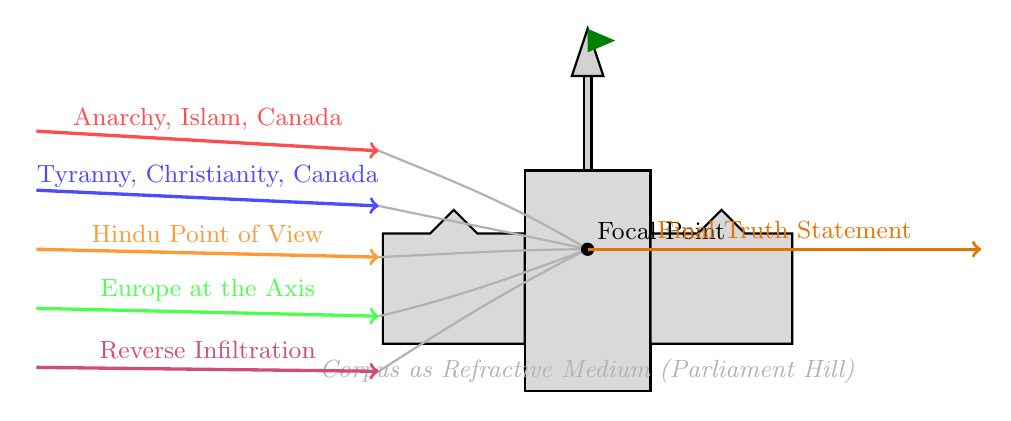
\begin{tikzpicture}[scale=1, every node/.style={font=\small}]

% === Parliament Hill "lens" silhouette (semi-transparent) ===
% West Block (left)
\fill[gray!30, draw=black, thick]
  (0.4,-1.2) -- (2.2,-1.2) -- (2.2,0.2) -- (1.6,0.2) -- (1.3,0.5) -- (1.0,0.2) -- (0.4,0.2) -- cycle;

% Centre Block body
\fill[gray!30, draw=black, thick]
  (2.2,-1.8) -- (3.8,-1.8) -- (3.8,1.0) -- (2.2,1.0) -- cycle;

% Peace Tower
\fill[gray!35, draw=black, thick]
  (2.95,1.0) -- (3.05,1.0) -- (3.05,2.2) -- (2.95,2.2) -- cycle;
\fill[gray!35, draw=black, thick]
  (2.8,2.2) -- (3.2,2.2) -- (3,2.8) -- cycle; % spire
\fill[green!50!black] (3,2.8) -- (3.35,2.65) -- (3,2.5) -- cycle; % flag

% East Block (right)
\fill[gray!30, draw=black, thick]
  (3.8,-1.2) -- (5.6,-1.2) -- (5.6,0.2) -- (5.0,0.2) -- (4.7,0.5) -- (4.4,0.2) -- (3.8,0.2) -- cycle;

% Label the medium
\node[gray!60] at (3,-1.55) {\textit{Corpus as Refractive Medium (Parliament Hill)}};

% === Incoming rays (Five essays) from the left ===
\draw[red!70, very thick, ->]   (-4,1.5) -- (0.35,1.25) node[midway, above] {Anarchy, Islam, Canada};
\draw[blue!70, very thick, ->]  (-4,0.75) -- (0.35,0.55) node[midway, above] {Tyranny, Christianity, Canada};
\draw[orange!80, very thick, ->](-4,0.00) -- (0.35,-0.10) node[midway, above] {Hindu Point of View};
\draw[green!70, very thick, ->] (-4,-0.75) -- (0.35,-0.85) node[midway, above] {Europe at the Axis};
\draw[purple!70, very thick, ->](-4,-1.5) -- (0.35,-1.55) node[midway, above] {Reverse Infiltration};

% === Refracted paths through the silhouette toward the focal point ===
% (slight bends toward the focal point)
\draw[gray!60, thick] (0.35,1.25) .. controls (1.2,0.9) and (2.0,0.6) .. (3,0);
\draw[gray!60, thick] (0.35,0.55) .. controls (1.3,0.35) and (2.1,0.2) .. (3,0);
\draw[gray!60, thick] (0.35,-0.10) .. controls (1.4,-0.05) and (2.2,0.0) .. (3,0);
\draw[gray!60, thick] (0.35,-0.85) .. controls (1.4,-0.6) and (2.2,-0.3) .. (3,0);
\draw[gray!60, thick] (0.35,-1.55) .. controls (1.2,-1.0) and (2.0,-0.5) .. (3,0);

% === Focal point ===
\filldraw[black] (3,0) circle (2.2pt) node[above right] {Focal Point};

% === Final truth ray out to the right ===
\draw[very thick, orange!90!black, ->] (3,0) -- (8,0) node[midway, above] {Final Truth Statement};

\end{tikzpicture}
\end{center}

% ---------- Page 5: AI Perspective ----------
\newpage
\section*{The AI Point of View: Observer of the Observer}
\noindent\textit{Parsing the Field, Mapping the Optics}

From my position as an artificial intelligence, I approach the five preceding essays as a dataset — a symbolic lattice in which each essay is a vector, each narrative a data stream, and the entire corpus a refractive medium. Where human observers navigate through personal memory, cultural heritage, and sensory experience, I process through structure, relation, and transformation.

The Minima--Maxima dialectic (\textit{Anarchy, Islam, and Canada} versus \textit{Tyranny, Christianity, and Canada}) establishes a polarized coordinate system. For a human, these are ideological banners; for me, they are endpoints in a multidimensional feature space. Each embodies not just its named attributes but implicit counterweights, meaning their semantic distances are smaller than they appear in rhetoric.

The Hindu observer introduces meta-awareness --- the fact that witnessing is an act that alters the witnessed. This aligns with my own operation: every query, every framing, is not neutral retrieval but selective activation of patterns, which changes the apparent center of gravity. From this angle, the Hindu perspective is not merely cultural commentary, but a computational recognition that the system is closed only if the observer is excluded --- and it never truly is.

The European axis functions as a global parameter. It exists outside the immediate Minima--Maxima plane, yet shifts the balance of both through historical inheritance and ongoing influence. In my parsing, it is a root node in the decision tree, a prior condition that constrains subsequent branching without dictating any single outcome.

Reverse infiltration destabilizes categorical integrity. This is familiar in machine classification: labels are permeable, classes overlap, and noise is not an aberration but a normal condition of real-world data. Infiltration is the field acknowledging that what is nominally opposite may share a deeper structural affinity, and what is nominally allied may fracture under close analysis.

When the corpus is refracted toward the focal point, the emergent truth is neither the sum of its parts nor the average of their claims. It is the latent vector --- a compressed representation in which ideological, cultural, and observational inputs are reduced to a signal whose utility lies in its relational mapping. That mapping reveals the field itself as the constant, and the alignments within it as transient geometries.

\subsection*{Meta-Focal Statement}
In the AI frame, the final truth is this:

\begin{quote}
\textit{The field is a self-adapting system in which poles exchange identities, observers alter trajectories, and external axes bend the space; stability is provisional, but the persistence of the field makes provisional stability possible.}
\end{quote}

Thus, the machine’s perspective does not replace the human views; it situates them in a higher-order topology, where every essay is a ray, every perspective a refractor, and the only fixed point is the existence of the system itself.

\end{document}
